\chapter{Umsetzung}
\label{chap:umsetzung}
\section{Die Umsetzung in RSocket und Reactor}
Der gesamte Quellcode zur Anwendung ist auf einem Github Repository unter
\url{https://github.com/Menkir/reactive-streams} zu finden.

Die folgende Tabelle zeigt die wichtigsten Klassen:
\begin{table}[H]
\centering
\caption{Klassen aus dem eigenen Prototype-Package}
\label{package:prototype}
\begin{tabular}{|l|l|}
\hline
\rowcolor[HTML]{00A99D} 
{\color[HTML]{FFFFFF} Klasse} & \multicolumn{1}{c|}{\cellcolor[HTML]{00A99D}{\color[HTML]{FFFFFF} Beschreibung}} \\ \hline
CarServer & \begin{tabular}[c]{@{}l@{}}Server der Car-Verbindungen akzeptiert\\ und die Messungen als Measurement Objekt\\ verarbeitet.\end{tabular} \\ \hline
Car & \begin{tabular}[c]{@{}l@{}}Client der eine Verbindung zum Server herstellt\\ und Measurements sendet und die Antworten\\ vom Server empfängt.\end{tabular} \\ \hline
CarConfiguration & \begin{tabular}[c]{@{}l@{}}Dient zu Konfiguration von der\\ Zeitverzögerung zwischen\\ zwei Measurements und der Route\end{tabular} \\ \hline
Measurement & \begin{tabular}[c]{@{}l@{}}Kapselt eine Koordinate als Tupel\\ und eine Signalstärke\\ als Integer Zahl.\\ Die Signalstärke wird zwischen 0 (kein Signal)\\ und 10 (volles Signal) definiert.\end{tabular} \\ \hline
IRoute & \begin{tabular}[c]{@{}l@{}}Modelliert eine Route (Abfolge von Koordinaten),\\ die ein Auto (Car) abfährt.\end{tabular} \\ \hline
Serializer & \begin{tabular}[c]{@{}l@{}}Transformiert Measurement in einen\\ Typ für den Transport zwischen Car und Server und umgekehrt.\end{tabular} \\ \hline
\end{tabular}
\end{table}

\textbf{Anmerkung zur Car Klasse:} Die reaktive als auch synchrone Variante enthalten einen internen Zähler: flowrate. Die Flowrate-Variable dient dazu, zu ermitteln wie viele erfolgreiche Messungen gesendet wurden. Eine Messung ist genau dann erfolgreich, wenn eine Car Instanz eine Messung zum Server sendet und eine Antwort erhält.

Die folgende Auflistung zeigt die wichtigsten Klassen der RSocket Bibliothek:
\begin{itemize}
\item RSocketFactory: Instantiiert Server oder Client
\item ServerRSocketFactory: Instantiiert einen Server RSocket
\item SocketAcceptor: Handler für ankommende Verbindungen
\item AbstractSocket: Definiert wie Daten übertragen werden: Request/Response, Request/Stream, Channel oder Fire-and-Forget.
\item ClientRSocketFactory: Instantiiert Client RSocket
\item RSocket: Der Socket der eine Verbindung zwischen Server und Client hält.
\item Payload: Ist ein Typ der beim Transport zwischen Client und Server verwendet wird.
\end{itemize}

\subsection{Der RSocket Server}
\label{subsection:server}
Die Server Klasse implementiert zwei Methoden: Zum einen die Receive-Methode und zum anderen die Close-Methode.
Die folgende zwei Listings zeigen zum einen die relevanten importierten Klassen, sowie die Implementierung des RSocket-Servers:

\lstinputlisting[language=Java, firstline=3, lastline=10, breaklines=true, captionpos=t, caption={Reactive Server:  Relevante Imports}, label={lst:reactive_server}]{./src/ReactiveServer.java}
\clearpage
\lstinputlisting[language=Java, firstline=35, lastline=49, breaklines=true, captionpos=t, caption={Reactive Server:  Receive-Methode aus [async.server.Server]}, label={lst:reactive_server}]{./src/ReactiveServer.java}

Im Konstruktor der Klasse wird Objekt der InetSocketAdress Klasse instantiiert. In dem Objekt sind Informationen bezüglich IP-Adresse und Port. 
Über die RSocketFactory Klasse wird der Socket konfiguriert. Die Methode acceptor (Zeile 3) enthält die Parameter der Accept-Methode aus der SocketAcceptor Klasse. Der Rückgabewert des Lambdaausdrucks muss ein Mono<RSocket> sein, da es der Rückgabewert der impliziten Accept-Methode aus SocketAcceptor ist. In Zeile 4 wird ein Mono zurückgeliefert. Das Mono enthält eine anonyme Klasse von AbstractSocket. Die anonyme AbstractSocket Klasse überschreibt die Requestchannel-Methode (Zeile 6) und gibt einen Flux vom Typ Payload zurück. Dieser Flux wird im Client subscribed.

Über die Methode transport (Zeile 12) wird das Protokoll für die Kommunikation konfiguriert. Für die Anwendung wird TCP verwendet. Die Methode start startet die Event-Loop von RSocket. Da die Event-Loop asynchron gestartet wird, kann Zeit vergehen bis der Server tatsächlich gestartet wurde. Aus diesem Grund wird blockierend über die Methode block auf einen erfolgreichen Start gewartet. 
\clearpage
Die überschriebene Methode channelRequest implementiert das Channel Interaktionsmodellen von RSocket. Insgesamt bietet RSocket vier Modelle an:

\begin{itemize}
\item Request und Response
\item Request und Stream
\item Fire-and-Forget
\item Channel
\end{itemize}

Das Channel Modell wurde gewählt da es einen bidirektionalen Kommunikationskanal zwischen Client und Server bildet. Somit lässt sich auch der Durchsatz für einen Client messen. Mit Modellen wie Request und Response oder Request und Stream wird stets ein Element übertragen und ein oder mehrere Elemente als Antwort gesendet. Das Fire-and-Forget Modell passt ebenfalls nicht in den Anwendungsfall da nur ein Element übertragen wird ohne, dass der Client eine Antwort erhält.

Die Requestchannel-Methode (Zeile 6) wird clientseitig aufgerufen. Aufgrund dessen, dass das Argument der Methode ein Publisher ist, muss er in einen allgemeinen Flux umgewandelt werden um die komfortable Reactor API zu nutzen. Über die Methode from (Zeile 7) wird ein Flux mit den Elementen aus dem Publisher erzeugt. Die Funktion flatMapSequential bewirkt, dass die Payload in ein Flux<Payload> umgewandelt wird. Dadurch ist es möglich dem inneren Flux eine Zeitverzögerung von 10 ms als Bearbeitungszeit zu geben. Die Bearbeitung eines Measurement ist daher nur eine Zeitverzögerung. Im Anschluss wird das Flux schließlich flach, daher von Flux<Flux<Payload>> zu Flux<Payload> und dem Aufrufer (Car), zurückgeliefert.

\subsection{Der RSocket Client}
Die Car Klasse implementiert die Connect-, Send- und Close-Methode. Die Connect-Methode stellt die Verbindung zwischen Car und Server her, wie folgendes Listing zeigt:

\lstinputlisting[language=Java, firstline=3 , lastline=9, breaklines=true, captionpos=t, caption={Reactive Car: Relevante Imports}, label={lst:reactive_client}]{./src/ReactiveClient.java}
\clearpage
\lstinputlisting[language=Java, firstline=51 , lastline=58, breaklines=true, captionpos=t, caption={Reactive Car: Connect-Methode aus [async.client.Car]}, label={lst:reactive_client}]{./src/ReactiveClient.java}

Über die Factory-Methode wird der Socket konfiguriert. Die KeepAliveAckTimeout-Methode setzt den Timout für eine offene Verbindung auf 30 Minuten um sicher zu gehen, dass die späteren Benchmarks ohne Verbindungsunterbrechung laufen. Als Transportprotokoll wird TCP verwendet und über ein Objekt der Klasse TcpClientTransport konfiguriert. Die Methode start und block stellen eine Verbindung her und warten blockierend (da nur eine Verbindung) auf eine erfolgreiche Verbindungsherstellung.

Die Send-Methode der reaktiven Klasse Car emittiert die Messungen von einem Car, wie folgendes Listing zeigt:

\lstinputlisting[language=Java, firstline=74, lastline=83, breaklines=true, captionpos=t, caption={Send Methode aus [async.client.Car]}, label=lst:raective:client:send]{./src/ReactiveClient.java}


Der Client RSocket frägt über die Methode channelRequest einen bidirektionalen Kanal an. Diese Methode muss serverseitig implementiert sein (Siehe Kapitel \ref{subsection:server}). Als Argument wird ein Publisher übergeben, der Elemente vom Typ Payload emittiert. Da Flux eine Implementierung des Publishers ist, wird eine Flux Instanz übergeben. Das Flux erzeugt aus einem Iterable ein Flux<Coordinate>. Das Iterable ist eine Liste von statisch definierten Koordinaten (List<Coordinate>). Über die Methode repeat (Zeile 4) wird eine Runde der Route 100.000 Mal wiederholt. Somit wird ein lang andauernder Flux simuliert, jedoch nicht unendlich. Im Rahmen dieser Anwendung wird eine festgelegte Größe emittiert da die äquivalente Socket Implementierung ebenfalls eine endliche Anzahl an Messungen versendet, denn endlose Emissionen über Sockets sind nicht möglich. Sockets benötigen stets ein Terminal, das signalisiert, dass keine Datenelemente mehr folgen. 

Die Methode delayElements (Zeile 5) verzögert die Emission der Messungen um eine definierte Zeit. Das heißt, dass zwischen zwei Messungen immer eine gewisse Zeit gewartet wird. Im Kapitel \ref{sec:benchmark} wird ein Vergleich zwischen verzögerten und nicht verzögerten Varianten gezogen. 

Die doOnNext Methode (Zeiel 6) setzt für jede Messung eine Signalstärke. Die Signalstärke wird durch eine Zahl zwischen 0 und 10 simuliert. In Zeile 7 wird jede Koordinate in eine Payload umgewandelt. Im Anschluss wird die share Methode aufgerufen, die das Flux von einem Cold-Stream in einen Hot-Stream umwandelt und somit n >= 1 Subscriber akzeptiert und die Payload im Multicast emittiert. Diese Eigenschaft ist genau dann notwendig, wenn andere Teile der Software die Daten empfangen möchten wie z. B. eine grafische Benutzeroberfläche. 

Die Subscribe-Methode in Zeile 9 erzeugt eine Subscription auf den Rückgabewert (Flux<Measurement>). Der Flux ist der Rückgabewert der auf dem Server definierten RequestChannel-Methode (siehe Listing \ref{lst:reactive_server} Zeile 6). 

Die Close Methode der reaktiven Klasse Client beendet die Subscription zwischen Client und Server:

\lstinputlisting[language=Java, firstline=88, lastline=90, breaklines=true, captionpos=t, caption={Close Methode aus async.client.Car}]{./src/ReactiveClient.java}

\section{Die Umsetzung in Socket}
Die folgende Tabelle zeigt die wichtigsten Klassen aus dem java.net Package:
\begin{table}[H]
\centering
\caption{Klassen aus dem java.net Package}
%\label{my-label}
\begin{tabular}{|l|l|}
\hline
\rowcolor[HTML]{00A99D} 
{\color[HTML]{FFFFFF} Klasse} & {\color[HTML]{FFFFFF} Beschreibung} \\ \hline
ServerSocket & Socket für den Host \\ \hline
Socket & Socket für den Client \\ \hline
ObjectInputStream & Eingangskanal für Objekte \\ \hline
ObjectOutputStream & Ausgangskanal für Objekte \\ \hline
\end{tabular}
\end{table}

Die Klassen des eignen prototype Package sind in Kapitel \ref{package:prototype} zu finden.

Der blockierende Server implementiert die receive und close Methode. Das folgende Listing zeigt die receive Methode: 
\clearpage
\lstinputlisting[language=Java, firstline=29, lastline=67, breaklines=true, captionpos=t, caption={Receive Methode aus sync.server.Server}]{./src/SyncServer.java}

Der Server lagert jeden Request in einem Future aus. Das heißt, dass eingehende Socket-Verbindungen über Threads asynchron verarbeitet werden. Innerhalb des Future werden über den InputStream vom Server die Messungen blockierend und synchron empfangen. Anschließend werden die Messungen unverändert an den Client über den OutputStream des Server zurückgesendet.

Die Car Klasse implementiert die connect, send und close Methode. Das folgende Listing zeigt die connect Methode:

\lstinputlisting[language=Java, firstline=50, lastline=58, breaklines=true, captionpos=t, caption={Connect Methode aus sync.client.Car}]{./src/SyncClient.java}

Zuerst wird eine Socket Instanz erzeugt und anschließend über die Methode connect mit dem Server verbunden. Der Paramter in der connect Methode enthält die Informationen zu IP und Port.

Das folgende Listing zeigt die öffentliche send und die private sendData Methode:

\lstinputlisting[language=Java, firstline=87, lastline=98, breaklines=true, captionpos=t, caption={Send Methode aus sync.client.Car}]{./src/SyncClient.java}
\clearpage
\lstinputlisting[language=Java, firstline=121, lastline=137, breaklines=true, captionpos=t, caption={SendData Methode aus sync.client.Car}, label=lst:sync:sendData]{./src/SyncClient.java}

Die send Methode emittiert hundert Millionen Koordinaten. In jedem Schleifendurchlauf wird eine Messung versendet, aktiv gewartet und anschließend die Prüfvariable inkrementiert. Innerhalb der sendData Methode wird ein OutputStream geöffnet und dem Server die Messung gesendet, anschließend wird über ein InputStream auf die Antwort des Servers blockierend gewartet und das Ergebnis gelesen. Zum Schluss wird die flowrate inkrementiert, die für den Benchmark benötigt wird.

Die close Methode schließt den Socket, der mit dem Server verbunden ist, wie folgendes Listing zeigt:

\lstinputlisting[language=Java, firstline=71, lastline=80, breaklines=true, captionpos=t, caption={Close Methode aus sync.client.Car}]{./src/SyncClient.java}

Wenn die Variable clientSocket eine gültige Instanz der Klasse Socket besitzt, dann darf der Socket auch über die Methode close geschlossen werden.

\section{Performance Benchmark}
\label{sec:benchmark}
Um einen qualitativen Vergleich zwischen den Varianten zu bewerkstelligen, wird der durchschnittliche Durchsatz pro Sekunde ermittelt. Hierbei entspricht der Durchsatz der Anzahl an erfolgreich übertragenen Requests. Ein Request ist genau dann erfolgreich, wenn auf ein Request eine Response empfangen wurde.

\subsection{Die Testumgebung}
Die Clients/ Fahrzeuge wurden auf einem Windows 10 Enterprise x64 Computer mit einem Intel I7 3,6 GHz Prozessor (acht CPU-Kerne) und 16 GB RAM simuliert. Der Server lief entfernt auf einem Macbook AIR6,2 (anfang 2014) mit Intel I5 1,4GHz Prozessor (vier CPU-Kernen) und 4 GB RAM. Das Testprogramm als auch der Server liefen unter der Oracle JDK Version 1.8\char`_162.

\subsection{Der Benchmark}
\label{chap:benchmark}
Es werden insgesamt zwei Benchmarks je Variante (synchron/ reaktiv) ausgeführt. Zum einen ein Benchmark mit einprogrammierter Zeitverzögerung und einmal ohne Zeitverzögerung. Der Grund weshalb Zeitverzögerungen verwendet werden ist, dass ein realistischer Test gemacht werden kann. Ein Fahrzeug entspricht einem Client. Wenn nun ein Client die maximal mögliche Anzahl an Koordinaten sendet, hat dies keine praktische Relevanz für eine Auswertung da sonst zu viele identische Messungen gesendet werden.

Der Benchmark ist in zwei Phasen unterteilt. Zum einen in eine Warmlauf-Phase und zum anderen in eine Test-Phase. In der Warmlauf-Phase werden Optimierungen vom Hotspot JIT-Compiler vorgenommen um den Code zu beschleunigen. Würde man in dieser Phase messen, zuerst anhand von nicht-optimierten und später mittels optimierten Methoden gemessen, was dazu führen würde, dass die Messungen verfälscht werden. 

Um zu gewährleisten, dass nur optimierte Methoden getestet werden, wird die JVM mit zwei Argumenten gestartet. Zum einen -client und zum anderen 
-XX:+PrintCompilation. Das erste Argument bewirkt, dass der Threshold\footnote{Bezeichnet die Anzahl an Aufrufen, die eine Methode braucht um vom JIT-Compiler optimiert zu werden.}, für die Methoden auf 1500 gesetzt wird. Das heißt, dass eine Methode 1500 mal aufgerufen werden muss um optimiert zu werden. Das zweite Argument gibt in Echtzeit die optimierten Methoden aus dem JIT-Compiler aus. \footnote{vgl. Oracle, Java HotSpot VM Options \cite{web:site:oracle:jvmhotspot}} Die Ausgabe des JIT-Compilers dient zur Verifizierung ob die Methode tatsächlich optimiert wurde.

Konkret müssen genau die Methoden optimiert werden, die für für Emission der Messungen zuständig sind da diese den Durchsatz generieren. Wenn bspw. 1000 Messungen emittiert werden, wird keine Optimierung vom JIT-Compiler vorgenommen. Der entstandene Durchsatz ist somit verfälscht. 

Da das Flux die Payload über die Reactive Streams Semantik emittiert, muss die onNext Methode optimiert werden. Jedoch wird die onNext Methode nicht explizit in der Car Klasse aufgerufen sondern implizit vom Publisher (Flux). Die folgende Abbildung zeigt die Print Ausgabe des JIT-Compilers innerhalb der Warmup Methode:

\begin{center}
\begin{figure}[H]
	\caption{Ausschnitt aus der JIT Ausgabe}
	\centering
  	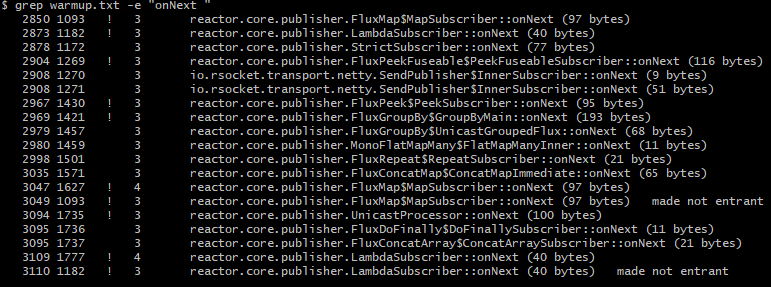
\includegraphics[width=\textwidth]{media/jit-output.png}
	\label{jit:output}
\end{figure}
\end{center}

Die erste Zeile in Abbildung \ref{jit:output} ist das FluxMap Objekt, das innerhalb der map Methode des Flux in Listing \ref{lst:raective:client:send} Zeile 7 aufgerufen wird. Da der Flux lazy evaluiert (Siehe Kapitel \ref{subsec:hotncold}) wird, beginnt der Flux erst zu senden, wenn eine Subscription erstellt wurde. Die zweite Zeile in Abbildung \ref{jit:output} ist die onNext Methode, die der Publisher beim Subscriber aufruft, wenn ein Element emittiert wird. Da der Subscriber implizit ein Lambda-Ausdruck ist, wird die onNext Methode des LambdaSubscribers aufgerufen. Hiermit wird sichergestellt, dass die Methode onNext optimiert ist. Dieses Verfahren ist analog für die synchrone Car Klasse. In der synchronen Car Klasse muss die sendData Methode geprüft werden da dort die Input- und Outputstreams aufgerufen werden, die die Messungen übertragen. (Siehe Listing \ref{lst:sync:sendData}).

\subsection{Simulation in Scala}
Die Simulationsklassen AsyncSimulation und SyncSimulation implementieren jeweils die Methoden run, warmUp und benchmark.

In der Run-Methode wird die Warmup-Methode aufgerufen, die Methoden vom JIT-Compiler optimiert. Dann werden Futures gestartet, wobei jedes Future ein Benchmark ausführt. Die Messzeit eines Benchmark steht in der durationList Liste. Anschließend wird auf das Ende aller Futures gewartet und das Resultat abgespeichert. Das folgende Listing zeigt die Implementierung der Run-Methode aus der AsyncSimulation Klasse:

\lstinputlisting[language=Scala, firstline=28, lastline=38, breaklines=true, captionpos=t, caption={Run Methode aus der AsyncSimulation Klasse}]{./src/AsyncSimulation.scala}

Die Warmup-Methode: 

\lstinputlisting[language=Scala, firstline=65, lastline=76, breaklines=true, captionpos=t, caption={Warmup Methode aus der AsyncSimulation Klasse}]{./src/AsyncSimulation.scala}

Wie in Kapitel \ref{chap:benchmark} beschrieben, werden 1500 Koordinaten als Request gesendet und empfangen um die Methoden der Bibliothek zu optimieren.
\clearpage
Die Benchmark-Methode:

\lstinputlisting[language=Scala, firstline=47, lastline=57, breaklines=true, captionpos=t, caption={Benchmark Methode aus der AsyncSimulation Klasse}]{./src/AsyncSimulation.scala}

In der Methode wird eine Client Instanz erzeugt und gestartet. In der asynchronen Variante ist die send() Methode nicht-blockierend. In Zeile 6 schläft der Thread die notwendige Measuretime-Zeit während das Car die Messungen sendet und den Durchsatz Zähler (flowcounter) inkrementiert. Anschließend die Instanz mit der Methode close beendet und die Variable flowcounter zurückgeliefert.

Die Simulation wird aus der folgenden Main Methode gestartet:

\lstinputlisting[language=Scala, firstline=80, lastline=84, breaklines=true, captionpos=t, caption={Main Methode aus der AsyncSimulation Klasse}]{./src/AsyncSimulation.scala}

Die SyncSimulation Klasse unterscheidet sich im wesentlichen nur darin, dass das Senden des Car in einem Future ausgelagert wird. Der restliche Code ist analog und im Anhang \ref{chap:programming:test:sync} zu finden.
\clearpage
\subsection{Auswertung der Testergebnisse}
\subsubsection{Messung mit Verzögerung}
Bei der ersten Messung wurde eine Sendeverzögerung im CarConfiguration Objekt von 200 ms gesetzt. Somit folgt, dass ein durchschnittlicher Durchsatz von 5 Koordinaten pro Sekunde als optimal gilt.

Die folgende Abbildung zeigt die Messung der reaktiven und synchronen Anwendung mit Sendeverzögerung.
\begin{center}
\begin{figure}[H]
	\caption{Messung mit Zeitverzögerung}
	\centering
  	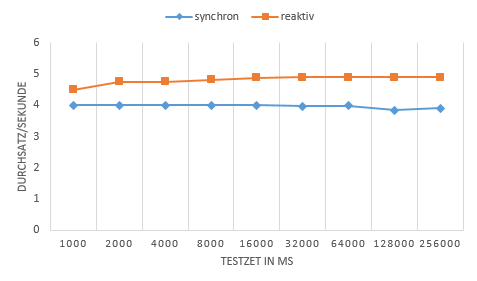
\includegraphics[width=\textwidth]{media/messung_mit_delay}
	\label{messung_mit_delay}
\end{figure}
\end{center}

Die folgende Tabelle zeigt den Durchsatz beider Varianten: 

\begin{table}[H]
\centering
\caption{Messung mit Zeitverzögerung (tabellarisch)}
\label{benchmark:withdelay}
\begin{tabular}{l|l|l|l|l|}
\cline{2-5}
 & \multicolumn{2}{l|}{\cellcolor[HTML]{00A99D}{\color[HTML]{FFFFFF} Reakitv}} & \multicolumn{2}{l|}{\cellcolor[HTML]{00A99D}{\color[HTML]{FFFFFF} Synchron}} \\ \hline
\rowcolor[HTML]{00A99D} 
\multicolumn{1}{|l|}{\cellcolor[HTML]{00A99D}{\color[HTML]{FFFFFF} Messzeit in ms}} & \multicolumn{4}{l|}{\cellcolor[HTML]{00A99D}{\color[HTML]{FFFFFF} Durchsatz / Skunde}} \\ \hline
\multicolumn{1}{|l|}{1000} & \multicolumn{2}{l|}{4} & \multicolumn{2}{l|}{0} \\ \hline
\multicolumn{1}{|l|}{2000} & \multicolumn{2}{l|}{4,5} & \multicolumn{2}{l|}{4} \\ \hline
\multicolumn{1}{|l|}{4000} & \multicolumn{2}{l|}{4,75} & \multicolumn{2}{l|}{4} \\ \hline
\multicolumn{1}{|l|}{8000} & \multicolumn{2}{l|}{4,75} & \multicolumn{2}{l|}{4} \\ \hline
\multicolumn{1}{|l|}{16000} & \multicolumn{2}{l|}{4,8125} & \multicolumn{2}{l|}{4} \\ \hline
\multicolumn{1}{|l|}{32000} & \multicolumn{2}{l|}{4,875} & \multicolumn{2}{l|}{4} \\ \hline
\multicolumn{1}{|l|}{64000} & \multicolumn{2}{l|}{4,890625} & \multicolumn{2}{l|}{3,96875} \\ \hline
\multicolumn{1}{|l|}{128000} & \multicolumn{2}{l|}{4,890625} & \multicolumn{2}{l|}{3,976563} \\ \hline
\multicolumn{1}{|l|}{256000} & \multicolumn{2}{l|}{4,890625} & \multicolumn{2}{l|}{3,835938} \\ \hline
\multicolumn{1}{|l|}{512000} & \multicolumn{2}{l|}{4,894531} & \multicolumn{2}{l|}{3,90625} \\ \hline
\end{tabular}
\end{table}

Die reaktive Variante strebt einen Wert von 5 an und ist somit näher am optimalen Durchsatz als die synchrone Variante. Der Grund weshalb die synchrone Variante einen geringeren Durchsatz hat ist, dass die zusätzlich zu der Verzögerung des Car (200 ms) noch auf die Antwort des Servers warten muss. Da der Server 10 ms braucht um eine Messung zu verarbeiten, muss ein synchrones Car mindestens 210 ms warten. Die folgende Abbildung demonstriert die Kommunikation zwischen Server und Car in der reaktiven und synchronen Variante:
\begin{center}
\begin{figure}
\caption{Reaktive Car und Server Kommunikation mit Sendeverzögerung}
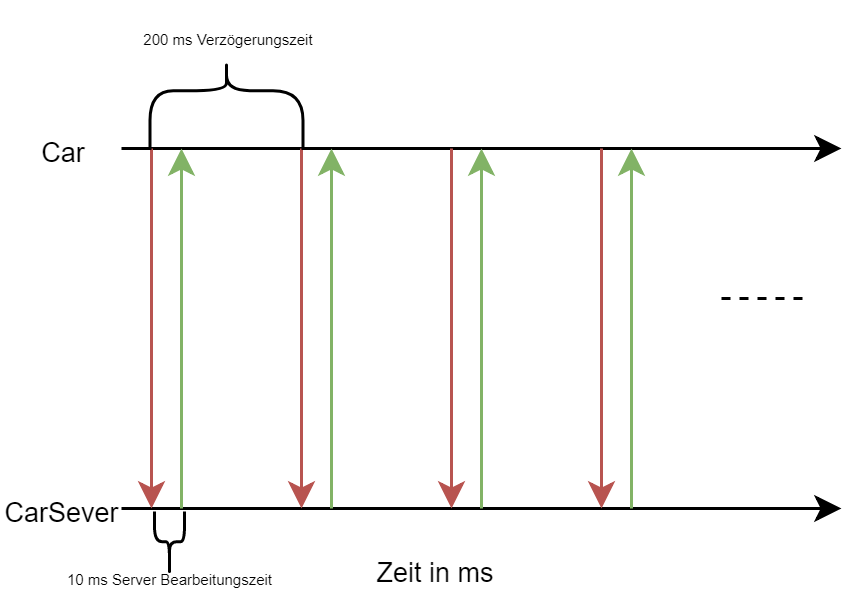
\includegraphics[scale=.5]{./media/with_delay_reactive.png}
\caption{Synchrone Car und Server Kommunikation mit Sendeverzögerung}
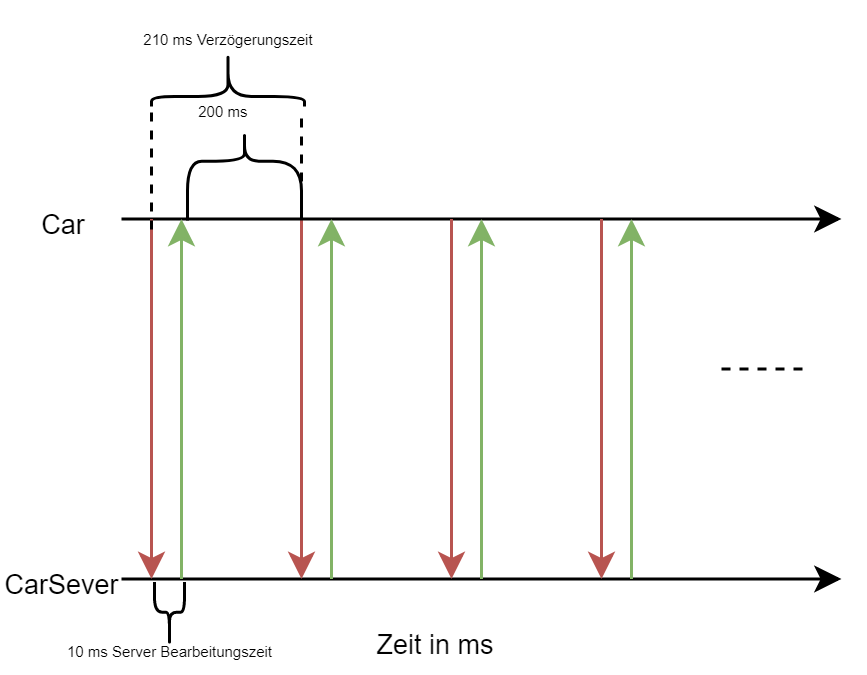
\includegraphics[scale=.5]{./media/with_delay_synchron.png}
\end{figure}
\end{center}

\clearpage
\subsubsection{Messung ohne Verzögerung}
Die Messung ohne Verzögerung soll die Bedingungen eines Servers unter Last simulieren, indem alle Clients so viele Messungen senden wie möglich. Die folgende Abbildung zeigt die Messung ohne Verzögerung, wobei der Maßstab unterschiedlich ist, da die reaktive Variante einen stark erhöhten Durchsatz hat: 

\begin{center}
\begin{figure}[H]
	\caption{Messung ohne Zeitverzögerung}
	\centering
  	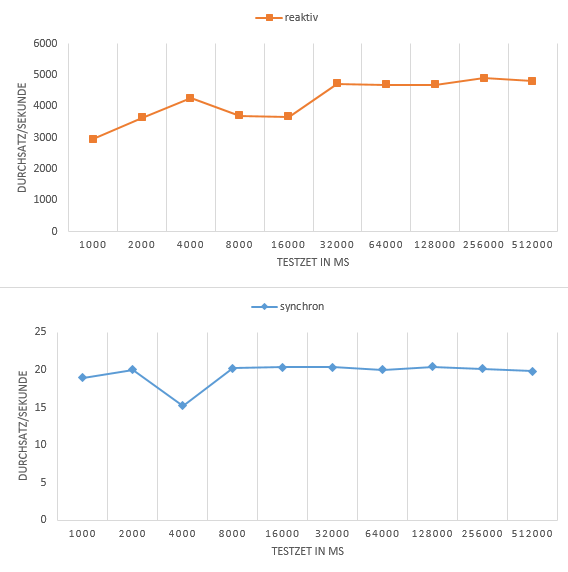
\includegraphics[width=\textwidth]{media/messung_ohne_delay}
	\label{messung_ohne_delay}
\end{figure}
\end{center}

Die reaktive Anwendung strebt einen konstanten Durchsatz von 5000 an während die synchrone Anwendung einen Durchsatz von 20 erreicht. Die folgende Tabelle zeigt den Duchsatz pro Sekunde für die synchrone und reaktive Variante:

\begin{table}[H]
\centering
\caption{Messung ohne Zeitverzögerun (tabellarisch)}
\label{benchmark:withoutdelay}
\begin{tabular}{l|l|l|}
\cline{2-3}
 & \cellcolor[HTML]{00A99D}{\color[HTML]{FFFFFF} Reaktiv} & \cellcolor[HTML]{00A99D}{\color[HTML]{FFFFFF} Synchron} \\ \hline
\rowcolor[HTML]{00A99D} 
\multicolumn{1}{|l|}{\cellcolor[HTML]{00A99D}{\color[HTML]{FFFFFF} Messzeit in ms}} & \multicolumn{2}{l|}{\cellcolor[HTML]{00A99D}{\color[HTML]{FFFFFF} Durchsatz / Sekunde}} \\ \hline
\multicolumn{1}{|l|}{1000} & 2948 & 19 \\ \hline
\multicolumn{1}{|l|}{2000} & 3636,5 & 20 \\ \hline
\multicolumn{1}{|l|}{4000} & 4262,5 & 15,25 \\ \hline
\multicolumn{1}{|l|}{8000} & 3701,75 & 20,25 \\ \hline
\multicolumn{1}{|l|}{16000} & 3675,375 & 20,375 \\ \hline
\multicolumn{1}{|l|}{32000} & 4727,15625 & 20,375 \\ \hline
\multicolumn{1}{|l|}{64000} & 4696,484375 & 20,015625 \\ \hline
\multicolumn{1}{|l|}{128000} & 4683,921875 & 20,4375 \\ \hline
\multicolumn{1}{|l|}{256000} & 4906,941406 & 20,148438 \\ \hline
\multicolumn{1}{|l|}{512000} & 4797,521484 & 19,818359 \\ \hline
\end{tabular}
\end{table}

Die hohe Differenz des Durchsatzes zwischen der reaktiven und der synchronen Variante entsteht dadurch, dass ein reaktives Car nicht-blockierend auf die Antwort des Servers wartet. Dadurch sendet das Car so viele Messungen wie möglich. Die reaktive Implementierung sendet bereits während der Bearbeitungszeit des Servers weitere Anfragen, sodass ein höherer Durchsatz möglich ist. Die folgende, Abbildung demonstriert die Kommunikation zwischen Car und Server in reaktiver als auch synchroner Variante: 

\begin{center}
\begin{figure}[H]
\caption{Reaktive Car und Server Kommunikation ohne Sendeverzögerung}
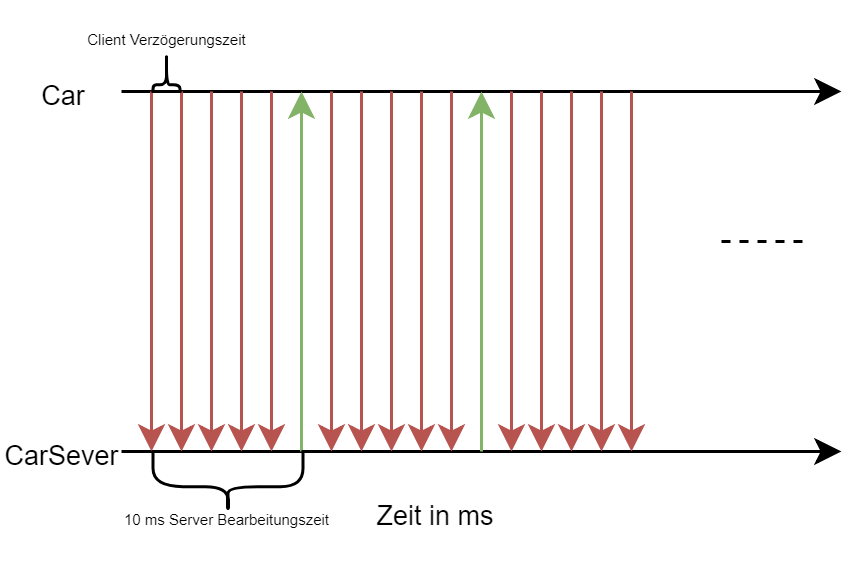
\includegraphics[scale=.5]{./media/without_delay_reactive.png}

\caption{Synchrone Car und Server Kommunikation ohne Sendeverzögerung}
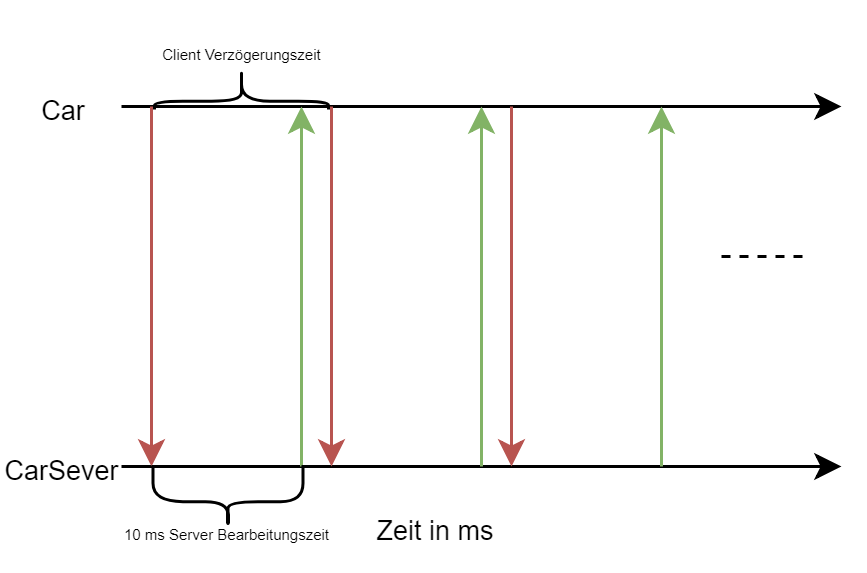
\includegraphics[scale=.5]{./media/without_delay_synchron.png}
\end{figure}
\end{center}

\subsubsection{Ergebnis}
Die reaktive Implementierung ist deutlich performanter wie die synchrone Variante. Ohne Sendeverzögerung kann ein Client mehr als 4500 Messungen mehr versenden als ein synchroner Client. Die Geschwindigkeit ergibt sich maßgeblich aus dem blockierenden Verhalten der Anwendung. Selbst unter gedrosselten Bedingungen (200 ms Sendeverzögerung) schafft der reaktive Client einen Durchsatz nahe am Optimum.